\scanpage{255}
\mspage{775}

Let on the other hand, in the case where $X$ is differentiable at $x$, \deleted{\unsure{Germ}}
\[
\tag{76}
\uline{\unsure{\mathrm{Germarc\,diff}|\mathrm{Courarc\,diff}}}(X,x)
\]
be the full subcategory of \deleted{$\unsure{\mathcal C_x|\mathcal G_x}$} $\uline{\unsure{\mathrm{Germarc}|\mathrm{Courarc}}}(X,x)$ formed by the differentiable germs of arcs. Let $\mathbb S_x$ \inserted{$\simeq\mathbb S^1$} be \deleted{the category}\inserted{the }space of half-lines of the Tangent space $\mathrm{Tang}_x(X)$
\[
\tag{77}
\mathbb S_x=
\begin{array}{l}
\inserted{\text{space of}}\\
\text{Half-lines}\\
\text{of }\mathrm{Tang}_x(X)
\end{array}
\simeq\mathbb S^1,
\]
and let us consider the fundamental groupoid
\diagram{\begin{tikzcd}[column sep=large]
{\text{(78)}\quad\Pi_1(\mathbb S_x)} \arrow[r,"\approx"] & \uline{\mathrm{Rev\,uni}}(\mathbb S_x).
\end{tikzcd}}

\margin{\figure{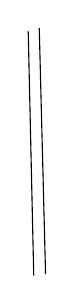
\begin{tikzpicture}[x=1cm,y=1cm]
\draw (0,0) -- (0.07,-3.1);
\draw (0.14,0.04) -- (0.22,-3.08);
\end{tikzpicture}}}
I am going to define an equivalence of categories
\diagram{\begin{tikzcd}[column sep=large,row sep=large]
{\text{(79)}\quad\uline{\unsure{\mathrm{Germarc\,diff}|\mathrm{Courarc\,diff}}}(X,x)} \arrow[r,"\approx"] \arrow[d,"\approx"{rotate=90}] &
\Pi_1(\mathbb S_x) \arrow[d,"\approx"{rotate=90}]\\
\uline{\mathrm{Rev\,uni}}(D_x^*) & \uline{\mathrm{Rev\,uni}}(\mathbb S_x)
\end{tikzcd}}
which, on the sets of objects, is to be the map \unsure{associating} to $\forall$ differentiable germ of an arc at $x$ its half-\uline{tangent}. The question is thus, if $\gamma,\gamma'$ are two such arcs, corresponding to half-tangents $\Delta,\Delta'$, to define a canonical bijection


\scanpage{256}

\margin{\figure{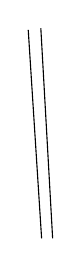
\begin{tikzpicture}[x=1cm,y=1cm]
\draw (0,0) -- (0.17,-2.65);
\draw (0.16,0.02) -- (0.31,-2.65);
\end{tikzpicture}}}
\diagram{\begin{tikzcd}[column sep=huge,row sep=large]
{\text{(80)}\quad\mathrm{Isom}(\gamma,\gamma')} \arrow[r,"\sim"] \arrow[d,equal,"\mathrm{d\acute ef}"] &
\mathrm{Isom}_{\Pi_1\mathbb S_x}(\Delta,\Delta') \arrow[d,equal,"\mathrm{d\acute ef}"]\\
\mathrm{Isom}(D_{x,\gamma}^{*\sim},D_{x,\gamma'}^{*\sim}) &
{\begin{array}{l}
\text{classes of paths}\\
\text{in }\mathbb S_x^*\text{ from }\Delta\\
\text{to }\Delta'
\end{array}}
\end{tikzcd}}

\deleted{\illegible{1}}
Instead of defining the bijection (80) directly, I am going to define rather a functor (which will be an equivalence of categories)
\diagram{\begin{tikzcd}[column sep=large]
{\text{(81)}\quad\Theta:\Pi_1(\mathbb S_x)} \arrow[r,"{(\deleted{\unsure{\to|\sim}}\approx)}"] &
\uline{\mathrm{Rev\,uni}}(D_x^*),
\end{tikzcd}}

Let \deleted{$\mathcal A$}
\[
\tag{82}
\left\{
\begin{array}{l}
\mathcal A_x\text{ set of }\inserted{\text{closed}}\text{ }1\text{-connected subsets of }\mathbb S_x\\
(\text{i.e. }\uline{\text{arcs}}\text{ of a circle in }\mathbb S_x,\\
\quad\unsure{\text{possibly}}\text{ reduced }\unsure{\text{to}}\text{ points,}\\
\quad\text{but }\ne\mathbb S_x)
\end{array}
\right.
\]
this is an ordered set, \unsure{and one|thus} \deleted{the set} defines an ordered category $\uline{\mathcal A}_x$ (the objects are the $\in\mathcal A_x$, the arrows are the inclusions) --- and we know that the enveloping groupoid \inserted{$\uline{\mathrm{Gr}}(\uline{\mathcal A}_x)$} of this ordered category is canonically equivalent to $\Pi_1(\mathbb S_x)$,


\scanpage{257}
\mspage{776}

more precisely, let \deleted{$\unsure{\uline{\mathcal A}_{0x}|\uline{\mathcal A}_x}$}\inserted{$\uline{\mathrm{Gr}}_0(\uline{\mathcal A}_x)$} be the full subcategory of $\uline{\mathrm{Gr}}(\uline{\mathcal A}_x)$ (whose set of objects is $\mathcal A_x$) whose objects are the \uline{one-point} arcs, \& we then have a canonical equivalence
\diagram{\begin{tikzcd}[column sep=large]
{\text{(83)}\quad\uline{\mathrm{Gr}}_0(\uline{\mathcal A}_x)} \arrow[r,"\approx"] & \Pi_1(\mathbb S_x)
\end{tikzcd}}
which on objects reduces to $\{a\}\longmapsto a$, and which, for any arc \deleted{$\unsure{\mathbb S|\xi}$} $A$ with endpoints $a,b$, whence inclusion isomorphisms \unsure{in|in} $\uline{\mathrm{Gr}}(\mathcal A_x)$
\diagram{\begin{tikzcd}[column sep=normal,row sep=large]
{\text{(84)}\quad\raisebox{-1.6em}{$\left\{\rule{0pt}{3.2em}\right.$}} &
a \arrow[r,"\sim"] & A & b \arrow[l,"\sim"'] & \\
& \text{whence}\quad a \arrow[rr,"\sim"] & & b & \text{in }\uline{\mathrm{Gr}}(\mathcal A_x)
\end{tikzcd}}
associates to this arrow $a\overset{\sim}{\longrightarrow}b$ of $\uline{\mathrm{Gr}}_0(\mathcal A_x)$ the arrow of $\Pi_1(\mathbb S_x)$, defined by the arc $A$ regarded as a path from $a$ to $b$.

Thus, for $\forall$ groupoid $\mathcal G$, giving a functor
\diagram{\begin{tikzcd}[column sep=large]
{\text{(85)}\quad\Psi:\Pi_1(\mathbb S_x)} \arrow[r] & \mathcal G
\end{tikzcd}}
is equivalent to giving a functor

\scanpage{258}
\[
\tag{86}
\Psi : \underline{\mathcal A}_x \longrightarrow \mathcal G
\]
and (85) is an equivalence of categories iff
$\mathcal G$ is \deleted{\unsure{connected}} connected and
\deleted{\unsure{the}} its $\unsure{\pi_1|\Pi_1}$ is $\simeq\mathbb Z$, and if, for
\deleted{\unsure{an $x$ of}}\inserted{a pair $(a,b)$ of}
distinct points $a,b$ of $\unsure{\mathbb S_x}$, defining two arcs $A$ and $B$
with endpoints $a,b$, \deleted{of}considering the automorphism of $a$ in
$\underline{\mathrm{Gr}}_0(\mathcal A_x)$ i.e. in
$\underline{\mathrm{Gr}}(\mathcal A_x)$, composed of
\[
\tag{86bis}
\diagram{\begin{tikzcd}[column sep=small]
\{a\} \arrow[r,"\sim"] & A & \{b\} \arrow[l,"\sim"'] \arrow[r,"\sim"] & B & \{a\} \arrow[l,"\sim"']
\end{tikzcd}}
\]
the corresponding automorphism of $\Psi(\{a\})$ in $\mathcal G$
is a \uline{generator} of $\mathrm{Aut}_{\mathcal G}(\Psi(\{a\}))$.

We are thus going to define a functor
\[
\tag{87}
\underline{\mathcal A}_x \longrightarrow
\underline{\mathrm{Revuni}}(D_x^*)
\]
\deleted{and} (satisfying the additional condition stated).
To define such a functor, it suffices to define a functor
\[
\tag{88}
\underline{\mathcal A}_x \longrightarrow
\begin{gathered}
\text{category of 1-connected germs}\\
\text{of spaces, \unsure{over|over} the}\\
\text{germ }D_x^*
\end{gathered}
\]

\scanpage{259}
\mspage{777}
by composing this functor with the functor
\[
\tag{89}
\begin{gathered}
\text{category of 1-connected germs}\\
\text{of spaces \unsure{over|over}}\\
\text{the germ }D_x^*
\end{gathered}
\longrightarrow \underline{\mathrm{Revuni}}(D_x^*).
\]
In fact, (88) \unsure{will associate|we associate} to $\forall\ A\in
\deleted{\unsure{\mathcal E}}\mathcal A_x$ a
\deleted{germ of a \unsure{subspace} of $X$ at $x$, of which}
\inserted{filter on $X-x$ tending to $x$, of which}
we will take the germ \deleted{\unsure{residual}}.

\deleted{\unsure{The half-lines}}
\inserted{The elements \inserted{$A$} of}
$\mathcal A_x$ are obviously identified with the \uline{cones}
\deleted{\unsure{open}}\inserted{closed $C$}
in $\mathrm{Tang}_x(X)$, \deleted{\unsure{disti}}
distinct from $\{0\}$ and from the
\inserted{\unsure{tangent$^{\mathrm t}$|tangent}} space $\forall$ entire.
\deleted{\unsure{Let $C$ be a}}
\inserted{Let $\unsure{C\mathcal A_x|C\in\mathcal C\mathcal A_x}$ be one of these cones.}
Let us consider a local isomorphism
\deleted{\unsure{a}}
\[
\tag{90}
f:(\mathrm{Tang}_x(X),0)\deleted{\unsure{\&}}
\xrightarrow{\sim}(X,x),
\]
\deleted{whose map}
\inserted{whose map} on tangent spaces is the identity.
\deleted{When} If $C$ is a cone $\in\mathcal C\mathcal A_x$,
its image under such an isomorphism depends on the choice of the local isomorphism in question.
But let us consider the \deleted{\unsure{family|set of}}
\inserted{filter base}
\deleted{\unsure{arcs}}\inserted{of} cones
\inserted{$C'\in\mathcal C\mathcal A_x$} containing
\deleted{$\unsure{\in}$} $C$ \uline{strictly}
(i.e. corresponding to arcs $A'$ which are \uline{neighborhoods}
of $A$, or again such that $C'-\{0\}$ is a neighborhood of
$C\setminus\{0\}$), then the

\scanpage{260}
\deleted{germ of spaces defined by the base}
\inserted{the image under (90) \deleted{\unsure{of this}}
\inserted{of the filter defined by the} base of a}
filter on $\mathrm{Tang}_x(X)$ formed by the
$V\cap(C'\setminus\{0\})$ \unsure{, where|:} $V$
ranging over the neighborhoods of $0$ in $\mathrm{Tang}_x(X)$,
is a filter on $X\setminus\{x\}$ which no longer depends on the choice of $f$,
and which tends to $x$, hence defines a germ of spaces
\inserted{$\widetilde A$ or $\widetilde C$}
over \deleted{$\unsure{X_x|X}$} $D_x^*$.
This germ of spaces, \deleted{\unsure{is é|and it}}
isomorphic to the germ of spaces defined by $\mathrm{Tang}_x(X)$ endowed with the filter
with base the $V\cap(C'-\{0\})$ --- where one can take $V$
convex closed \unsure{symmetric|symmetric}, hence
$V\cap(C'-\{0\})$ contractible --- is obviously 1-connected.
For $A$ i.e. $C$ varying \unsure{i.e.} for $A_1\subset A_2$
i.e. $C_1\subset C_2$ we have the corresponding inclusion relation
\inserted{\deleted{$\unsure{A}$}
\diagram{\begin{tikzcd}
\widetilde C_1 \arrow[r] & \widetilde C_2
\end{tikzcd}}}
on the germs of spaces in $D_x^*$.
We thus do get (88), whence (87)\inserted{and (81)}, and we check
that the latter is indeed an equivalence of \deleted{categories}
groupoids, via the \unsure{verification|verification$^{\mathrm t}$}
\deleted{\unsure{by}} \unsure{made explicit|made explicit} above ((86bis)).

\scanpage{261}
\mspage{778}
Let us now consider, once again, a differentiable arc $\gamma$ in $X$
issuing from $x$, and its half-tangent $\Delta$.
Then $\{\Delta\}\in\mathcal A_x$, and we can consider the germ
of spaces $\{\Delta\}^{\sim}$ over $D_x^*$.
We have \inserted{\unsure{the|some}} two canonical inclusion morphisms
\[
\tag{91}
\diagram{\begin{tikzcd}
\gamma \arrow[r,hook] & \{\Delta\}^{\sim} \arrow[r,hook] & D_x^*
\end{tikzcd}}
\]
and we deduce from this a canonical isomorphism
\[
\tag{92}
\diagram{\begin{tikzcd}[column sep=large]
\mathrm{Revuni}(D_x^*,\gamma) \arrow[r,phantom,"\simeq"] \arrow[d,equal,"\mathrm{déf}"]
& \mathrm{Revuni}(D_x^*,\{\Delta\}^{\sim}) \arrow[d,equal,"\mathrm{déf}"] \\
D_{x,\gamma}^{*\sim} & \Theta(\Delta)
\end{tikzcd}}
\]
If $\gamma'$ is another differentiable arc at $x$, corresponding to the half-tangent
$\Delta'$, we thus have
\[
D_{x,\gamma}^{*\sim}\simeq\Theta(\Delta),\qquad
D_{x,\gamma'}^{*\sim}=\Theta(\Delta')
\]
whence
\[
\diagram{\begin{tikzcd}[column sep=large,row sep=large]
\mathrm{Isom}(D_{x,\gamma}^{\unsure{*}\sim}\unsure{\}},D_{x,\gamma'}^{*\sim})
\arrow[r,phantom,"\simeq"] \arrow[d,equal,"\mathrm{déf}"]
& \mathrm{Isom}(\Theta(\Delta),\Theta(\Delta')) \\
\mathrm{Isom}(\gamma,\gamma')
& \mathrm{Isom}_{\Pi_1(\mathbb S_x)}(\Delta,\Delta')
\arrow[u,"\sim","\Theta"']
\end{tikzcd}}
\]
which is the \deleted{\unsure{right}} bijection (80) sought.

\deleted{Let} In summary, we have an essentially commutative diagram of equivalences
of groupoids